\chapter{Concepts}
\label{chapter:concepts}

We discuss the various concepts discussed in the thesis scope in this chapter.

\section{Paxos}
\label{section:concepts.paxos}

The consensus algorithm used in the system is Paxos \sectionref{paxos}.
\citet{Robbert2011} is the specific paper referred to for the implementation of
Warlock. This section describes the specific flavor of the algorithm.

The processes of the group can be classified into different roles based on the
part of algorithm they are responsible for.

\begin{itemize}
    \iterm{Replica}: Replicas are processes responsible for assigning proposal
    number to an operation and handle decisions made.
    \iterm{Acceptor}: Acceptors are the ``memory'' of the algorithm. They keep
    track of which leader is currently in-charge to issue commands.
    \iterm{Leader}: Leaders receive proposals from replicas and they try to
    co-ordinate the messaging to acceptors for that proposal. It uses ballots%
    \sidenote{
      \emph{Ballots} are monotonically increasing ids that are unique to a
      specific leader. Each leader has an infinite number of ballots.
    }
    to track the execution order or proposals.
    \iterm{Scout}: A scout process is spawned by the leader to active a specific
    ballot.
    \iterm{Commander}: A commander process is spawned by the leader to try
    and get votes for a specific proposal.
\end{itemize}

Assuming the scout was already run and the current leader has its ballot as the
largest one, lets see a typical flow of the proposal from its initiation to its
execution skipping on the smaller details and corner cases.

\begin{itemize}
    \item A proposal is created by the client based on the request. This
      proposal is uniquely identified and contains all the necessary request
      information. This proposal is sent to the replica.
    \item The replica checks if the proposal is a duplicate and if not it
      assigns a sequence number%
      \sidenote{
        The replica is responsible for maintaining a consistent log of
        operations. This log is made up of slots with each of the slots
        indexed by a sequence number.
      }
      to it before sending it off to the leader.
    \item The leader, which already has run the scout, spawns a commander with
      the ballot and proposal information.
    \item The commander sends out a message to all acceptors with the ballot
      information to all acceptors asking them to approve the proposal.
    \item The acceptors respond positively if it has not seem another larger
      ballot number and negatively otherwise.
    \item The commander waits for a quorum (usually a majority of total
      acceptors) of acceptors. Once it has received majority of the approvals,
      the commander asks all the replicas to execute the proposal and exits.
    \item The replica checks if the received decision is the next index on
      the consistent log and executes the proposal if it is.
\end{itemize}

In the above use case we see the routing for one instance of individual
processes running. There will be several simultaneously running processes. The
routing in the algorithm is as follows.

\begin{itemize}
  \item The client broadcasts its command to all the replicas.
  \item Each of the replica sends a ``propose'' message to all the leaders.
  \item The leader sends the P1a message to all the acceptors via the scout.
  \item The acceptor only replies to the sender with a P1b message.
  \item On quorum acceptance from a quorum of acceptors, the leader sends
    ``accept'' message (P2a) to all the acceptors via the commander.
  \item The acceptors responds with P2b only to the sender.
  \item The leader on quorum response, broadcasts the decision to all the
    replicas.
  \item Each of the replica replies to the client.
\end{itemize}

The paper details several optimizations to make the algorithm more practical.

\section{Erlang}

Erlang \citep{erlang} is a virtual machine based general purpose functional
programming language built by Ericsson mainly to develop telephony applications
\citep{Armstrong07}. Erlang was build to handle large number of network
requests with special attention given to handling failures.

A process is the concurrency primitive of Erlang. Each of the processes are
isolated and have access to their own private memory. This allows us to build
large scale applications with the Actor model%
\sidenote{
  An actor is a process that can
  \begin{inparaenum}[(i)]
    \item Send messages to other actors.
    \item Spawn new actors.
    \item Specify the behaviour to be used when it receives its next message.
  \end{inparaenum}
}
\citep{Clinger81}.

Erlang also supports hot code loading%
\sidenote[3]{
  \emph{Hot code loading}: Dynamically updating running software.
}
which allows us to upgrade the system's
code without restarting or disrupting the service.

The ideas of concurrency, fault tolerance, distributability, hot code loading
behind Erlang maps well on to the building large web applications.

\todo{Add and arrange features}

\todo{define modules, processes}

\todo{define ets, dict}

\section{Open Telecom Platform}
\label{section:concepts.otp}

Open Telecom Platform (\abbr{OTP}) is a collection of Erlang libraries.
The \abbr{OTP} code is
well tested, robust and provide design patterns allowing us to quickly build
Erlang applications. We take a look at few of the principles from \abbr{OTP}
that is used in the project.

\subsection{Supervision}
\label{section:concepts.supervision}

Supervisors are processes that monitor workers processes and restart them based
on a predefined set of rules. An application can be designed in the form of a
tree with fine grained control to handle crashing processes and to localize such
crashes. A typical Erlang supervisor tree looks like
\figureref{supervision.tree}.

\begin{figure}
  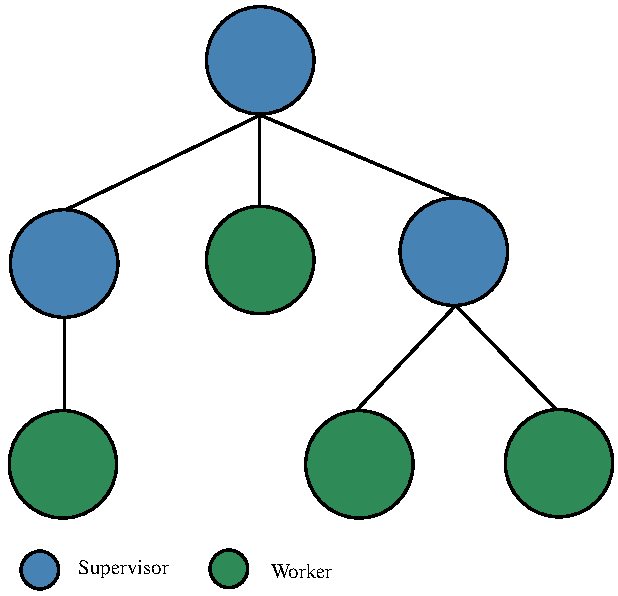
\includegraphics[width=0.5\wholewidth]{supervision-tree}
  \caption[Supervision Tree]{%
    Supervision Tree: Structure of a typical Erlang supervision tree.}
  \label{figure:supervision.tree}
  \normalcaption
\end{figure}

A process as per the supervision tree can either be a supervisor%
\sidenote{
  \emph{Supervisor}: An Erlang process responsible for creating, terminating,
  monitoring and restarting processes as defined.
}
or a worker%
\sidenote[3]{
  \emph{Worker}: A worker process in this context is any other process started
  by the supervisor that is not a supervisor itself.
}. Processes that crash are restarted by the supervisor as per its
restart strategy%
\sidenote[6]{
  \emph{Restart Strategy}: This defines how the supervisor should restart
  crashed children.
  \begin{inparaenum}[(i)]
    \iterm{One for one}: Only the crashed process is restarted.
    \iterm{One for all}: All the children under the supervisor are restarted if
    any of the process terminates.
    \iterm{Rest for one}: Similar to one for all, but children restart is based
    on just the first process.
    \iterm{Simple one for one}: Same as one for one, but the children are
    created dynamically.
  \end{inparaenum}
}
. The supervisor also provides several other options such as child
specifications, restart frequency, restart policy and so on to provide
fine grained control on the restart procedure.

\subsection{Behaviours}
\label{section:concepts.behaviours}
Behaviours are commonly used Erlang design patterns. They contain a predefined
set of functions necessary to implement specific design patterns allowing for
quick implementation.

The three main behaviours provided by the OTP library are

\begin{itemize}
    \iterm{gen\_server}: A process that waits for incoming events, performs
    actions based on the events and responds to the request.
    \iterm{gen\_event}: A process that acts as an event manager waiting for
    events to happen and runs specific event handlers based depending on it.
    \iterm{gen\_fsm}: A process that acts as a finite state machine.
\end{itemize}

\subsubsection{gen\_server}
\label{section:gen.server}

gen\_server is based on the typical architecture of client-server model
\citep{reliable.dist.sys}. It supports two types of requests viz, synchronous
calls%
\sidenote{
  \emph{Synchronous calls}: Also called blocking calls, has the caller wait till
  the process can provide a response.
}
and asynchronous calls%
\sidenote[2]{
  \emph{Asynchronous calls}: Also called non-blocking calls, is received by the
  process and handled when it has processed all the messages it had received
  before this request.
}
.

It also provides other features such as handling other types of messages (such
as \abbr{TCP}/\abbr{UDP} messages), hot code loading and sending requests to
other processes.

\subsection{Applications}
\label{section:concepts.applications}
Logical group of components can be glued together to form applications.
Applications have well-defined roles and Erlang provides convenient modules to
manage them.

\subsection{Releases}
\label{section:concepts.releases}
A release is a complete system packaged for deployment. Erlang provides modules
necessary to create packages for deploying new code and upgrading existing code.

\section{Erlang libraries}

A few external projects were used for building this system. We describe the
roles of these project.

\subsection{lager}

Lager \citep{lager} is a logging framework for Erlang applications. It provides
features such as fine grained log levels, multiple back end support, optimized
logging and relatively better performance.

\subsection{eredis}

eRedis \citep{eredis} is a non-blocking Erlang client library for Redis.

eRedis is used in this project to support the Redis back end and is used in the
implementation of Redis protocol support.

\subsection{Ranch}

Ranch \citep{ranch} is a socket acceptor pool for \abbr{TCP} protocols.

Ranch is used in this project for accepting and managing multiple client
connections for the Redis protocol implementation.

